\documentclass[]{article}
\usepackage{lmodern}
\usepackage{amssymb,amsmath}
\usepackage{geometry}                		% See geometry.pdf to learn the layout options. There are lots.
\geometry{letterpaper}                   		% ... or a4paper or a5paper or ... 
%\geometry{landscape}                		% Activate for rotated page geometry
%\usepackage[parfill]{parskip}    		% Activate to begin paragraphs with an empty line rather than an indent
\usepackage{graphicx}				% Use pdf, png, jpg, or eps§ with pdflatex; use eps in DVI mode
								% TeX will automatically convert eps --> pdf in pdflatex		
\usepackage[unicode=true]{hyperref}
\hypersetup{
            pdftitle={CC-BLAS.jl = Basic Sparse Linear Algebra for Topological Computing in Julia},
            pdfauthor={CVDLab},
            pdfborder={0 0 0},
            breaklinks=true}
\usepackage{listings}% http://ctan.org/pkg/listings
\lstset{
  basicstyle=\ttfamily,
  mathescape
}


%----macros begin---------------------------------------------------------------------
%\def\textbf#1{\alert{#1}}
%\def\emph#1{{\color{cyan}#1}}
\def\conv{\mbox{\textrm{conv}\,}}
\def\aff{\mbox{\textrm{aff}\,}}
\def\E{\mathbb{E}}
\def\R{\mathbb{R}}
\def\Z{\mathbb{Z}}
\def\N{\mathbb{N}}
\def\P{\mathbb{P}}
\def\v#1{{\bf #1}}
\def\p#1{{\bf #1}}
\def\T#1{{\bf #1}}
\def\vet#1{{\left(\begin{array}{cccccccccccccccccccc}#1\end{array}\right)}}
\def\mat#1{{\left(\begin{array}{cccccccccccccccccccccccccccc}#1\end{array}\right)}}

\def\lin{\mbox{\rm lin}\,}
\def\aff{\mbox{\rm aff}\,}
\def\pos{\mbox{\rm pos}\,}
\def\cone{\mbox{\rm cone}\,}
\def\conv{\mbox{\rm conv}\,}
\newcommand{\homog}[0]{\mbox{\rm homog}\,}
\newcommand{\relint}[0]{\mbox{\rm relint}\,}

\newtheorem{assignment}{Assignment}
\newtheorem{exercise}{Exercise}
\newtheorem{question}{Question}
\newtheorem{remark}{Remark}

\def\red#1{{\color{red} #1}}
\def\blue#1{{\color{blue} #1}}
\def\green#1{{\color{green} #1}}
\def\cyan#1{{\color{cyan} #1}}

%----macros end-----------------------------------------------------------------------------------

\title{%CC-BLAS.jl \(=\) 
Topology Computing w GraphBLAS Sparse Matrix Algebra
}
\author{F.~Milicchio$^a$, A.~Paoluzzi$^b$, 
 V.~Caravani$^a$, G.~DelMonte$^a$, O.~Elsayed$^a$, M.~Paolucci$^a$\\
\small{Department of \{Engineering$^a$, Mathematics and Physics$^b$\}, Roma Tre University, Rome, Italy}\\[3mm]
}

\date{\today}

\begin{document}
\maketitle


\begin{abstract}
In this paper we introduce a GraphBLAS implementation of sparse matrix methods to compute the topology of cellular complexes, using linear spaces of chains and linear operators of boundary and coboundary. Sparse matrices may be used to provide boundary representation of both solid models and/or their discretizations used in several scientific applications. Sparse matrices of such operators can be used within geometric methods of medical imaging, BIM, CAD, FEM, Computer Graphics, VR and AR, in order to efficiently compute multiple queries on incidence/adjacency of  cells, when using both decompositive, enumerative, boundary-based, manifold, and non-manifold representations of geometric models.
\end{abstract}

\tableofcontents


\section{Introduction}\label{introduction}
%=========================================

The aim of this paper is to introduce an approach to 2D and 3D
computational topology and geometry using a \emph{GraphBLAS} sparse matrix
representation of \emph{chain complexes} with linear operators $\partial_p$ and $\delta_{p-1} = \partial_p^\top$ between linear \emph{chain} spaces $C_p$:
\[ 
C_\bullet = (C_p, \partial_p) := 
C_3 \ 
\substack{
\delta_2 \\
\longleftarrow \\[-1mm]
\longrightarrow \\
\partial_3 
}
\ C_2 \ 
\substack{
\delta_1 \\
\longleftarrow \\[-1mm]
\longrightarrow \\
\partial_2 
}
\ C_1 \ 
\substack{
\delta_0 \\
\longleftarrow \\[-1mm]
\longrightarrow \\
\partial_1 
}
\ C_0 .
\] 
Let us to remark preliminary that when $p\in \{0,1\}$, a chain complex is a representation of a \emph{graph}, with $[\partial_1]$ the \emph{incidence matrix} between 1-chains (edges) in $C_1$ and 0-chains (vertices) in $C_0$. Also, the multiplication $[\partial_1][\delta_0]=[\partial_1][\partial_1]^t$ gives the \emph{adjacency} matrix of the graph, while the diagonal entries provide the degrees of vertices, defined by the number of incident edges on each vertex. The \emph{GraphBLAS} standard~\cite{GraphBLAS:standard} provides a small set of matrix primitives to compute graph properties that, combined together, allow for easy implementation of fast algorithms on large graphs.

In several application of computational geometry and topology---including
geo-mapping, building information modeling (BIM), medical imaging, CAD and
solid modeling, virtual and augmented reality, finite element modeling
and simulation (FEM, FEA), etc.---the amount and detail of 2D and/or 3D data
continue to grow. Analogously, the need for an unified approach to
graph algorithms and for unified and simplified interfaces, has been
well intercepted by the GraphBLAS initiative and the related 
standardization effort~\href{http://graphblas.org}{\texttt{graphblas.org}}. 
This paper aim is to show that the domaincovering of this standard library on graphs can be greatly extended, to cover the representation of more general \emph{cellular $d$-complexes} ($1\leq d\leq 3$) and their $p$-skeletons ($0\leq p\leq 3$).

(Co)chain complexes, as well (co)boundary operators, are well-known
basic tools of algebraic topology and homological algebra. In
particular, a \emph{chain complex} is a graded sequence of such linear
operators between graded linear spaces of ``chains''. A $p$-chain can be seen as a subset of a finite set $\texttt{V}$ of Euclidean points whose affine hull has dimension $p$.
Chain spaces and sparse matrices are the components of the Linear Algebraic
Representation (\texttt{LAR})~\cite{Dicarlo:2014:TNL:2543138.2543294}, that is being used for
boundary, decompositive, and enumerative
representations~\cite{Requicha:1980:RRS:356827.356833} of models of rigid solid objects.

Some numerical methods aiming to integrate domain modeling, differential
topology, mathematical modeling, and physical simulations were based on chains and
cochains, starting with~\cite{PALMER1995733,Palmer1993}. In particular,
Discrete Exterior Calculus (DEC) with simplicial complexes was
introduced by \cite{Hirani:2003:DEC:959640} and made popular by
\cite{Desbrun:2006:DDF:1185657.1185665,Elcott:2006:BYO:1185657.1185666}.
Finite Element Exterior Calculus 
(FEEC) is an advance in the mathematics of finite element 
methods~\cite{arnold_falk_winther_2006,Arnold:2010,Arnold:2018} that employs differential
complexes to construct stable numerical schemes. The Cell
Method~(CM) is a purely algebraic computational method
for modeling and
simulation~\cite{Tonti:1975,Tonti:2013,Ferretti:2014}
based on boundary/coboundary maps and a direct discrete formulation of
field laws. Our own research in geometrical and physical modeling with
chain and cochain complexes was introduced in
\cite{DiCarlo:2009:DPU:1629255.1629273,ieee-tase,Dicarlo:2014:TNL:2543138.2543294}.

More recently, we provided---using sparse
matrices---an algorithmic pipeline~\cite{TSAS:19} to compute the \emph{arrangement} of the
Euclidean \(d\)-space (\(d=2,3\)), i.e.~the partition of
it into a cellular \(d\)-complex, starting from a collection of (possibly intersecting) cellular
(\(d\)-1)-complexes embedded in \(\E^d\). In~\cite{paoluzzi2019finite} we
have shown that the \emph{atoms} of the Boolean algebra generated by
such space partition correspond one-to-one to the columns of the $[\partial_d]$ matrix
of the boundary operator \(\partial_d : C_d \to C_{d-1}\). This allows for fast
native reconstruction of every solid expression in the \emph{solid algebra} of
\(d\)-space generated by the input terms, usually called Constructive Solid Geometry (CSG)
in solid modeling~\cite{Requicha:1980:RRS:356827.356833}.

The topological background of linear chain spaces and chain complexes is summarized in 
Section~\ref{sec:background}, together with the concepts of boundary and coboundary linear maps between chain spaces.
In Section~\ref{chain-adjacencies-and-incidensies} an operational definition of topological queries through composition of operators corresponding to products of their sparse matrices is discussed.
In Section~\ref{boolean-algebras} an interpretation as a Boolean algebra of the partition of the Euclidean $d$-space produced by a collection of geometric objects is provided.
The implementation of such concepts using GraphBLAS is given in Section~\ref{graphblas-implementation}. Some simple examples of topology computation using linear algebra are shown in  Section~\ref{examples}.
In the Conclusion Section we briefly summarize our main points, state our findings, and propose some possible extension of this approach.

\section{Background}\label{background}
%===========================================================

Cellular complexes are largely used in Computer Graphics and in Geometric and Solid Modeling~\cite{Elter:10.1007/978-3-642-78114-8_12}. In particular, they provide the geometric-topological discretization for computer modeling and simulation of physical properties of both manmade and natural objects~\cite{DiCarlo:2009:DPU:1629255.1629273,ieee-tase}.

\subsection{Cell complexes vs Chain complexes}
\label{cell-complexes-vs-chain-complexes}
%--------------------------------------------

A \(p\)-chain can be seen as a subset of \(p\)-cells from a cellular
complex. The space of \(p\)-chains is closed
w.r.t.~addition and product times a scalar from a field. In particular, it is a linear (vector) space.

\paragraph{Cells and Chains}\label{sec:chain}
%------------------------------------------------------------------------------
%--
A $p$-\emph{manifold} is a topological space where each point has a neighborhood
that is homeomorphic to $\E^p$. A \emph{$p$-cell} $\sigma$ ($0\leq p\leq d$) of cellular complexes is piecewise-linear, connected, possibly non convex, $p$-manifold, and not necessarily contractible\footnote{The cells of CW-complexes are contractible to a point. With our LAR representation they may contain internal holes.}. An
$r$-face $\tau$ of a $p$-cell $\sigma$ ($0\leq r\leq p$) is an $r$-cell contained
in the frontier of $\sigma$.


A \emph{$p$-chain} can be seen, with some abuse of language, as a collection of $p$-cells.
The set $C=\oplus\ C_p$ of chains can be given the structure of a graded vector space  by
defining sums of chains with the same dimension, and products times scalars in a
field, with the usual properties.

A \emph{basis} $U_p$  is the set of \emph{independent} (or \emph{elementary}) chains $u_p \in C_p$, given
by singletons of $\Lambda_p$ elements. Every chain $c\in C_p$ is uniquely generated by
a linear combination of the basis with field coefficients. Once  the  basis is fixed, the coordinate
representation of each $\{\sigma_k\} = u_k \in C_p$ is unique. This is an ordered
sequence of coefficients, either from $\{0,1\}$ (unsigned representation) or from
$\{-1,0,+1\}$ (signed representation). With abuse of language, we
often call $p$-cells the independent generators of $C_p$, {i.e.}~the elements of
$U_p$.


\paragraph{Chain and cochain complexes}\label{graded-complexes}
%-------------------------------------------------------------------------------
%
A \emph{graded vector space} is a vector space $V$ expressed as a direct sum  of
spaces $V_k$ indexed by integers in $[0,d]$:
\[ V = \oplus_{k = 0}^d V_k, \qquad [0,d] := \{k\in\N \ |\ 0\leq k\leq d\}.
\]

A linear map $f:V\to W$ between graded vector spaces is called a \emph{graded
map} of degree $p\ $ if $f(V_k) \subset W_{k+p}$.

A \emph{chain complex} is a graded vector  space $V$ furnished with a graded
linear map $\partial : V \to V$ of degree $-1$ which satisfies $\partial^2 = 0$, called
\emph{boundary operator}. In other words, a chain complex
is a sequence of vector spaces $C_k$ and linear maps $\partial_k : C_k \to C_{k-1}$,
such that $\partial_{k-1} \circ\ \partial_{k} = 0$.

A \emph{cochain complex} is a graded vector space $V$ furnished with a graded
linear map $\delta : V \to V$ of degree $+1$ which satisfies $\delta^2 = 0$,
called \emph{coboundary operator}. That is to say, a cochain complex is a
sequence of vector spaces $C^k$ and linear maps $\delta^k : C^k \to C^{k+1}$,
such that $\delta^{k+1} \circ\ \delta^{k} = 0$.
%This duality implies that ... (Antonio !)

Since any linear map $L: V\to W$ between linear spaces induces a dual map $L': 
W' \to V'$ between their duals, any chain complex is associated with a dual 
cochain complex, and viceversa:
\[
(\delta^k \omega) g = \omega (\partial_{k+1} g), \qquad \omega \in C^k, g \in C_{k+1}.
\]
 In a Euclidean space, chain and cochain spaces can be trivially identified~\cite{ieee-tase}, so that we use the $C_p$ notation for both spaces, with $\partial_p: C_p\to C_{p-1}$, and $\delta_p = \partial_{p-1}^\top: C_{p-1}\to C_p$.


\section{Chain Adjacency and Incidence}
\label{chain-adjacencies-and-incidensies}
%=========================================

Boundary decompositions (B-reps) are the typical representations used in solid modeling and computer graphcs. The model boundary is partitioned into vertices (\texttt{V}: 0-cells), edges (\texttt{E}: 1-cells), and faces (\texttt{F}: 2-cells), where faces are often triangles or more general convex cells. 

\subsection{Boundary representation of solid models}
\label{boundary-representation-of-solid-models}
%--------------------------------------------------


In particular, a typical solid modeling representation employs some specialized data structure to efficiently traverse the boundary, moving from some element to the adjacent ones (with same dimension) or to incident ones (with different dimension). Several data structures have been used for this purpose~\cite{HofShapiro:2017}, taking into account both the efficiency of topological queries and the storage compactness. Three binary adjacency relations and six binary incidence relations can be needed by algorithms, as shown in Table~\ref{tab:relations}a.

Using chain operators, or better their matrices, when an ordering of elements has been fixed inside the sets \texttt{V}, \texttt{E}, and \texttt{F} using one-dimensional arrays, such binary relations can be represented and/or computed as shown in Table~\ref{tab:relations}b. It is easy to show (see Table~\ref{tab:relations}b), that all linear operators between chain spaces corresponding to binary relations between boundary elements can  be derived from $\partial_1$ and $\partial_2$ via matrix transposition or product over semirings~\cite{DBLP:journals/corr/KepnerABBFGHKLM16,GraphBLAS:API:2017}.

\begin{table}[htp]
\caption{(a) The 9 binary relations between boundary elements, and the 16 binary relations between decompositive elements; (b) corresponding linear operators between chain spaces. Remember that $\partial_p: C_p\to C_{p-1}$ and that $\delta_p = \partial_{p+1}^\top$. }
\begin{center}
\begin{tabular}{|c|ccc|c|}
\hline
 &\texttt{V} & \texttt{E} & \texttt{F} & \texttt{C} \\ 
\hline
\texttt{V} &\texttt{VV} & \texttt{VE} & \texttt{VF} & \texttt{VC} \\ 
\texttt{E} &\texttt{EV} & \texttt{EE} & \texttt{EF} & \texttt{EC} \\ 
\texttt{F} &\texttt{FV} & \texttt{FE} & \texttt{FF} & \texttt{FC} \\ 
\hline
\texttt{C} &\texttt{CV} & \texttt{CE} & \texttt{CF} & \texttt{CC} \\ 
\hline
\end{tabular}
$\qquad$
\begin{tabular}{|c|ccc|c|}
\hline
 &\texttt{$C_0$} & \texttt{$C_1$} & \texttt{$C_2$} & \texttt{$C_3$} \\ 
\hline
\texttt{$C_0$} & $[\partial_1][\delta_0]$ & $[\partial_1]$ & $[\partial_1][\partial_2]$ & $[\partial_1][\partial_2][\partial_3]$\\ 
\texttt{$C_1$} & $[\delta_0]$  & $[\delta_0][\partial_1]$ & $[\partial_2]$ & $[\partial_2][\partial_3]$ \\ 
\texttt{$C_2$} & $[\delta_1][\delta_0]$ & $[\delta_1]$ & $[\delta_1][\partial_2]$ & $[\partial_3]$ \\ 
\hline
\texttt{$C_3$} & $[\delta_2][\delta_1][\delta_0]$ & $[\delta_2][\delta_1]$ & $[\delta_2]$ & $[\delta_2][\partial_3]$ \\ 
\hline
\end{tabular}
\end{center}
\label{tab:relations}
\end{table}%


Note that we have assumed vectors as column matrices, so that an operator maps the column space to the row space of its matrix. Hence, in order to maintain the consistency between the two representations  we should read the relation $\texttt{AB} \subset \texttt{A}\times \texttt{B}$ as a map $\texttt{AB}: \texttt{B} \to \texttt{A}$.


\subsection{Space Decompositions}\label{space-decompositions}
%-------------------------------------------------------------
A similar representation scheme---called \emph{decompositive} in~\cite{Requicha:1980:RRS:356827.356833}---is also  used, both in solid modeling and in order to represent the domain decomposition in FEM and other discretizations of physical models. In this case a partition of the whole domain is provided, using cellular 3-complexes, given by \texttt{V}, \texttt{E}, \texttt{F}, and \texttt{C} sets of $0$-, 1-, 2- and 3-cells, where often the \texttt{C} elements  are either tetrahedra or hexahedra.  

For the topology of a graph (cellular 1-complex) just $C_0$ (vertices) and $C_1$ (edges) are needed, so that a complete representation is given by the signed or unsigned matrix $[\partial_1]$, corresponding to the relation $\texttt{EV} \equiv C_1\to C_0$.

It is worth noting that operators $\partial_1$, $\partial_2$, and $\partial_3$ are sufficient to represent the complete collection of $4\times 4$ operators (see Table~\ref{tab:relations}b), via matrix transposition or product over semirings. In other words, the \emph{chain complex} $C_\bullet = (C_p, \partial_p)$ of boundary matrices, $1\leq p\leq 1,2,3$ is a \emph{complete representation} of the topology of (a) graphs, (b) B-reps, and (c) decompositive representations, respectively. 

Cellular complexes may be either \emph{oriented} (signed) or \emph{non-oriented} (unsigned). In the first case the elements of operator matrices are taken over the domain $D=\{0,1\}$; in the second case they belong to the domain $D=\{-1,0,1\}$, so that passing from a coefficient $+1$ to a coefficient $-1$ (or viceversa) the element orientation is reversed.


\subsection{Minimal representations}\label{minimal-reps}

Most of earlier algorithms and procedures~\cite{
4055948,
Ala:1992:PAB:616022.617736,
Baumgart:1972:WEP:891970,
bowyer1995introducing,
bowyer1995svlis,
Braid:1975:SSB:360715.360727,
Brisson:1989:RGS:73833.73858,
cadanda,
Dobkin:1987:PMT:41958.41967,
Gomes:1999:MMB:304012.304039,
Guibas:1985:PMG:282918.282923,
HoffmannK01,
Kalay:1989:HET:63718.63719,
Lee:2001:PES:376957.376976,
Lienhardt:1991:TMB:115604.115610,
Mantyla:1988:ISM:60949,
Paoluzzi:1989:BAO:70248.70249,
Paoluzzi:1993:DMS:169728.169719,
Paoluzzi:1995:GPP:212332.212349,
Pascucci:1995:DCB:218013.218055,
Pratt94ashape,
Raghothama:1999:CUD:304012.304019,
Rap97,
RequichaVoelcker:77,
Rossignac:1991:CNG:115604.115606,
Rossignac:SGC:90,
Shapiro:1991:RSS:124951,
Shapiro:1995:PFS:218013.218029,
Silva:81,
Weiler:86,
Weiler:88,
Woo:85,
wozny1990geometric,
Yamaguchi:85,
yamaguchi1995ntb,
Zhou:2016:MAS:2897824.2925901,
bieri:95,
Rossignac:89,
Hoffmann:91,
Hoffmann:1989:GSM:74803,
Hoffmann:1987:RSO:866286} 
work with data
structures optimized for selected classes of geometric
objects. By contrast, our formulation, representation, and algorithms, cast in
terms of (co)chain complexes of (co)boundary maps, may be
applied to very different geometric objects, ranging from solid models
to engineering meshes, geographical systems, biomedical images.

Given a set $S=\{s_j\}$, the \emph{characteristic function} $\chi_A: S\to\{0,1\}$ takes value 1 for all elements of $A\subseteq S$ and 0 at all elements of $S$ not in $A$. 
We call \emph{characteristic matrix} $M$ of a collection of subsets $A_i\subseteq S$ ($i=1,\ldots,n$) the binary  matrix $M=(m_{ij})$, with $m_{ij} = \chi_{A_i}(s_j)$. {A  matrix $M_p$, whose rows are indexed by unit $p$-chains and columns are indexed by unit $0$-chains, provides a useful representation of a basis for the linear space $C_p$. Permuting (reindexing) either rows or columns provides a different basis.}   While chains are mostly presented as formal sums of cells, in the actual implementation their signed coordinate vectors are used as \emph{sparse} arrays, and in particular as CSC (Compressed Sparse Column) maps : $\N\to\{-1,0,1\}$.

It is possible to show~\cite{} that, when the $d$-cells are convex, the topology of a cellular $d$-complex is fully described by $M_{d-1}$ and by an embedding function $\mu: \texttt{V}\to \E^d$. When $d$-cells are more complex---say, non-convex or with holes---the triple $(M_{d-1}, M_{d-2}, \mu)$ is needed to get a full knowledge of the topology of the complex.

We call \texttt{LAR} (Linear Algebraic Representation) of subsets of a set \texttt{V} (vertices), the array, indexed by ordinals (one-to-one with subsets), of arrays of indices to \texttt{V} elements. This one is a compact representation of the \emph{characteristic matrix} of the collection of subsets.



\section{Sparse Matrices and Solid Boolean Algebras}\label{boolean-algebras}
%=================================================

Manuscript~\cite{paoluzzi2019finite} shows that the set of join-irreducible atoms of the Boolean Algebra generated by a partition of $\E^3$ are one-to-one with the basis of 3-chain space also generated by the partition, and hence with the columns of the $[\partial_3]$ matrix, which provides a boundary representation (as 2-cycles) of the independent elements of 3-space. 
An example of such space decomposition is shown in Figures~\ref{fig:image1} and~\ref{fig:image2}. The 3-cells are not in scale, and are suitably rotated to better exhibit their
complex structure, even containing internal holes. Their assembly gives the union of the five cubes. Each
\emph{3-cell is generated} as \emph{a column} of the \emph{sparse matrix} of
\emph{chain map} $\partial_3: C_3\to C_2$,  with values in $\{-1,0,1\}$.
They are the join-irreducible \emph{atoms} of the CSG algebra with closed regular cells.

\begin{figure}[htbp]
    \centering
    \begin{minipage}{0.475\textwidth}
        \centering
       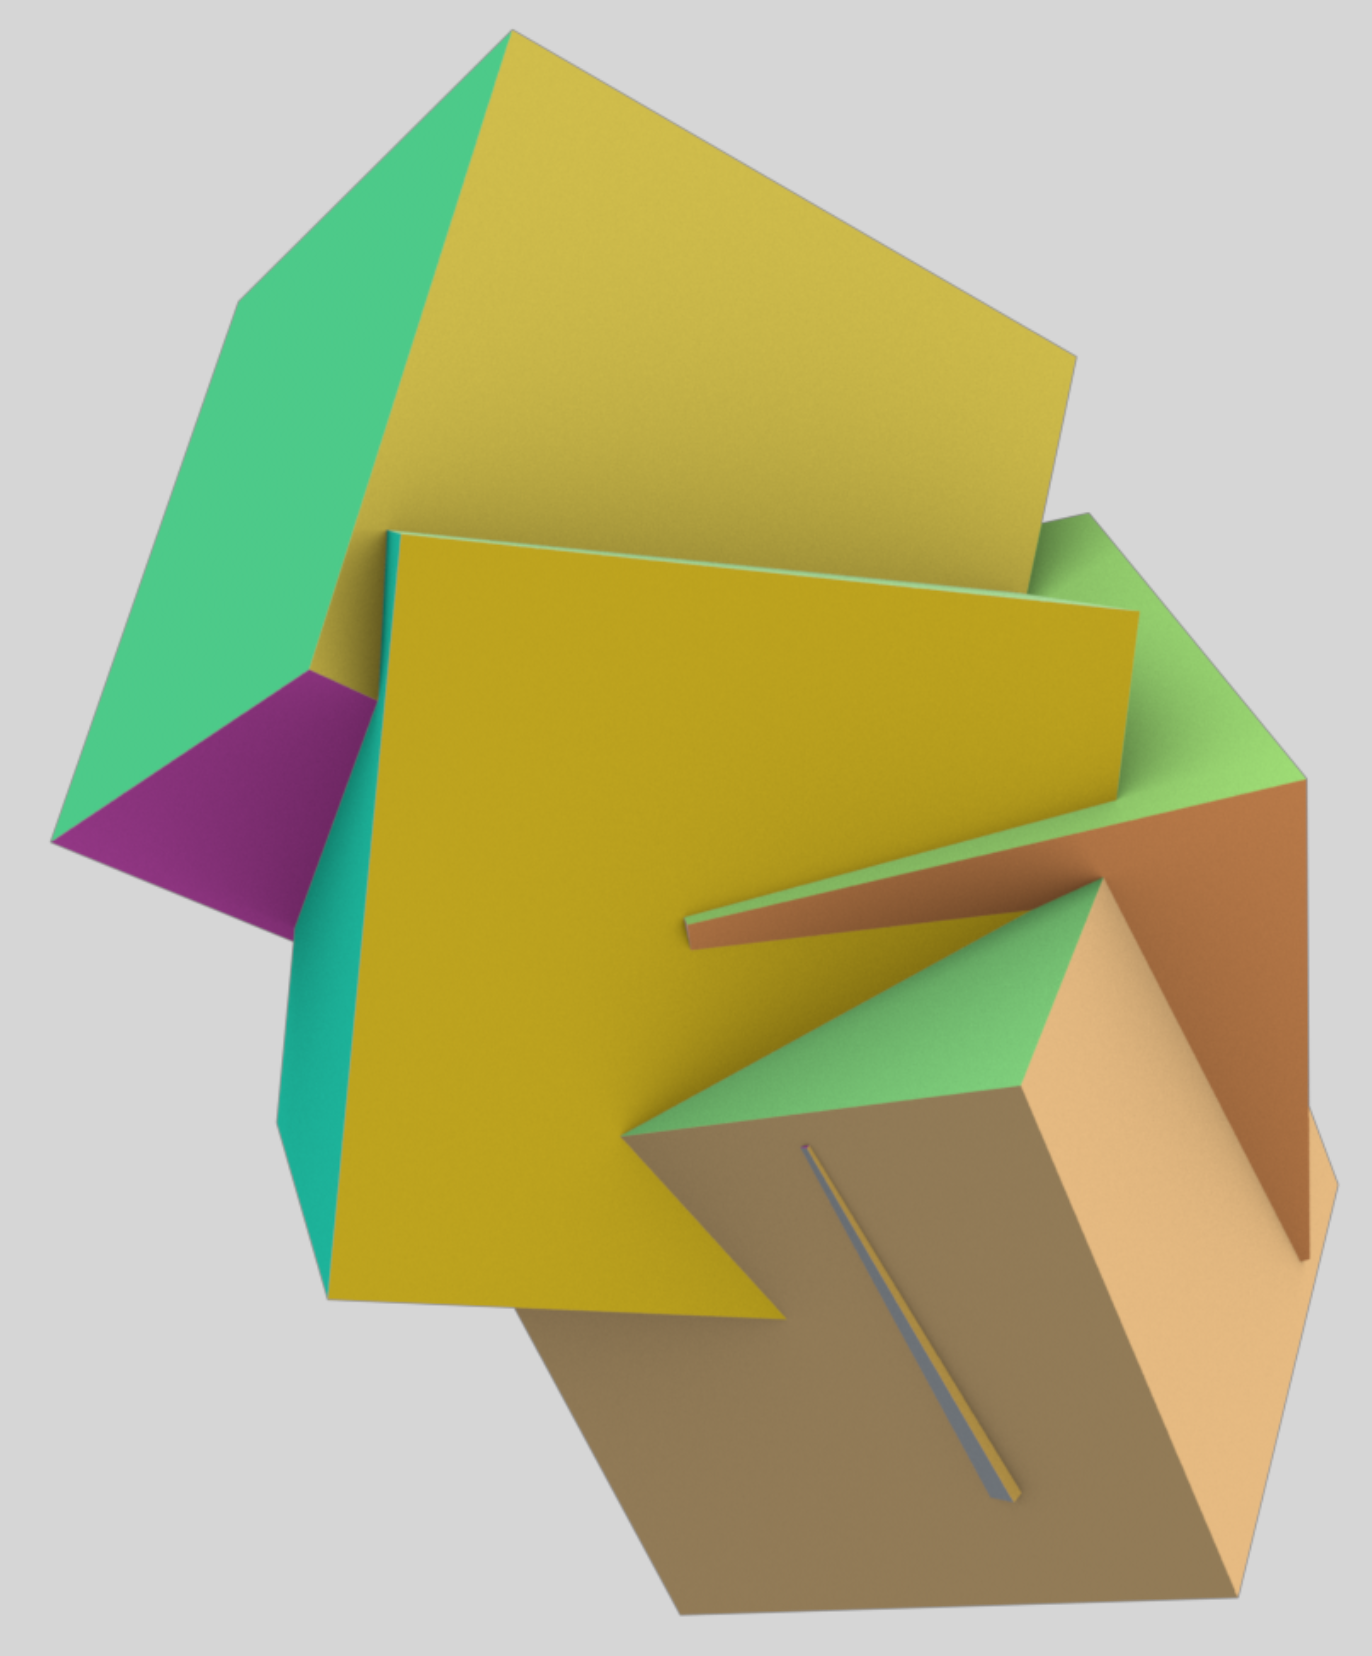
\includegraphics[width=0.6\linewidth]{../figs/image1.png} 
       \caption{A collection $\mathcal{S}$ of five random cubes in 3D Euclidean space.}
       \label{fig:image1}
    \end{minipage}\hfill
    \begin{minipage}{0.475\textwidth}
        \centering
       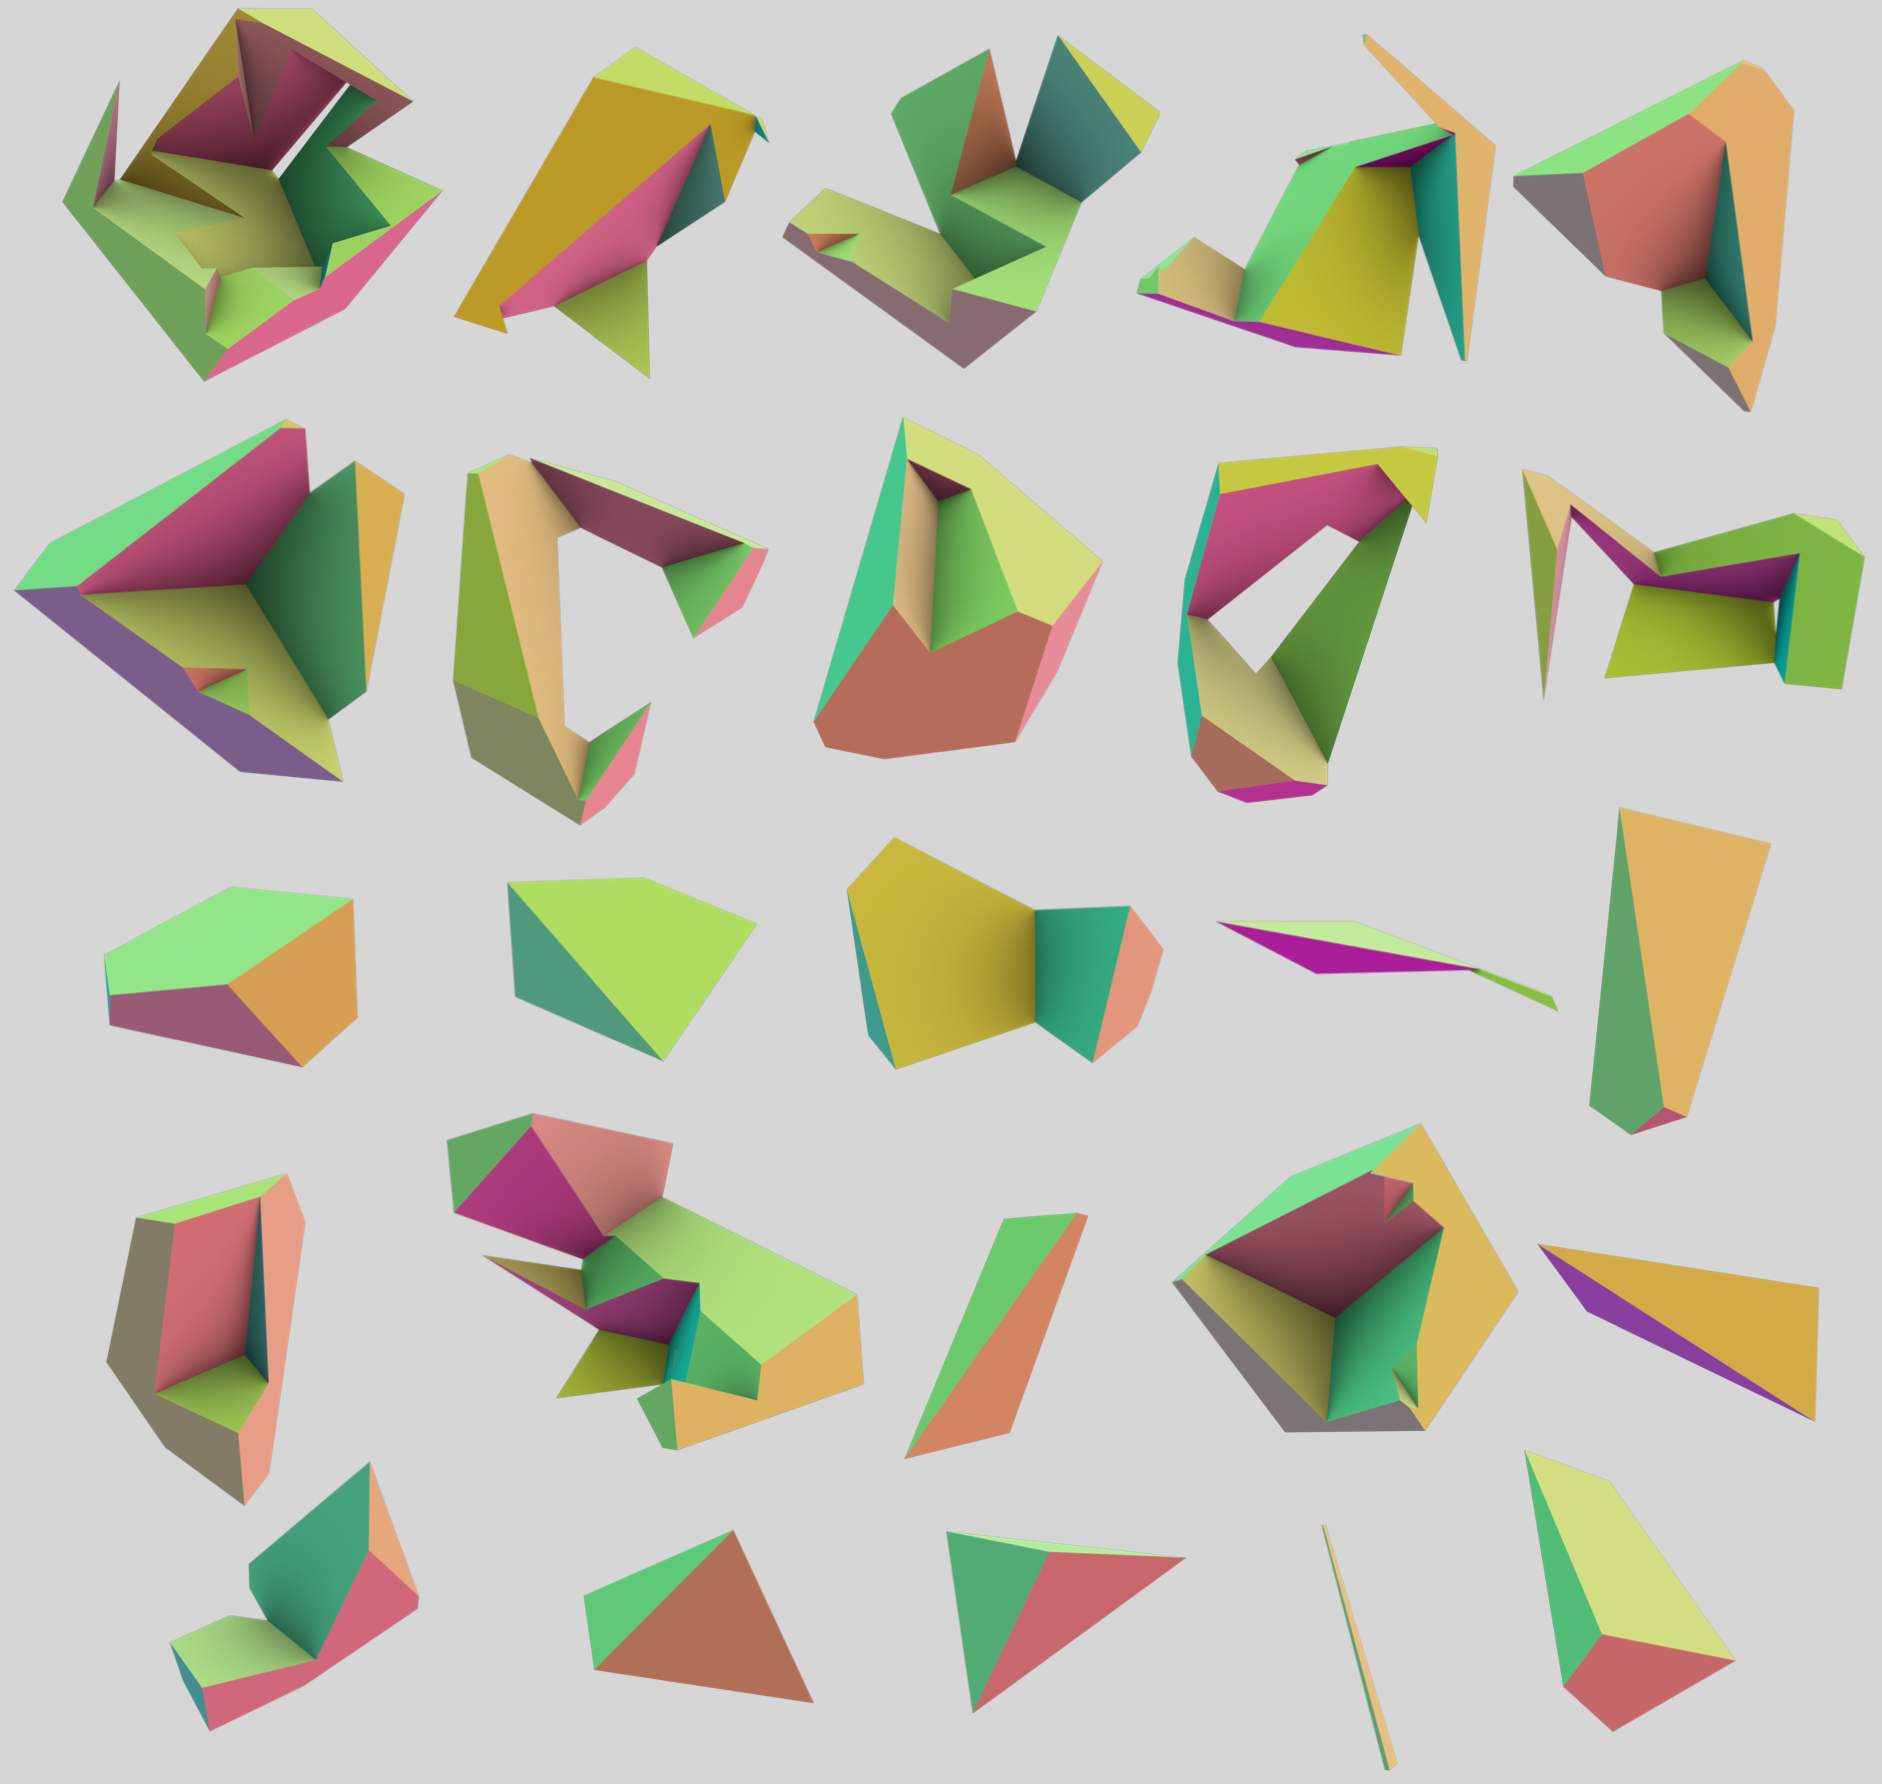
\includegraphics[width=0.8\linewidth]{../figs/image2.png} 
        \caption{3-cells of the generated arrangement $\mathcal{A}(\mathcal{S})$ of $\E^3$.
        They are given by columns of $[\partial_3]$ as \emph{atoms} of a solid Boolean algebra.}
       \label{fig:image2}
    \end{minipage}
\end{figure}

To generate the $d$-space arrangement induced by a collection of cellular ($d$--1)-complexes, some numerical algebra and basic tools of linear algebra and algebraic topology are used. In particular, (sparse) matrices of operators and matrix multiplication and transposition. Interval-trees and $kd$-trees are also introduced for acceleration of clustering of face cells into subsets of congruent shape. 

Using our approach with sparse matrices, the validity of topological computations is guaranteed, since these operator matrices must satisfy by construction the (graded) constraints: $[\partial_2][\partial_3]=[0]$ and $[\partial_1][\partial_2]=[0]$.  Similarly, we have $[\delta_1][\delta_0]=[0]$ and $[\delta_2][\delta_1]=[0]$.

With our approach based on boundary operators, the distinctions are removed between manifold and non-manifold representations (fairly standard in Solid Modeling), so allowing for mixing B-reps, cellular decompositions of elementary solids, and/or regular grids. This allows, e.g., for the generation of internal structures and mixed-dimensional objects needed in many applications, for example to make stronger and more resilient the ones to be produced via 3D printing.

Even more, the evaluation of CSG expressions of arbitrary complexity is done in a novel way, by combining the binary columns of 3D basis elements (i.e., the elements of the $U_3$ basis) with native Julia's operators for bitwise operations. In other words, once the $3$-space partition is generated, and $3$-cells are classified w.r.t.~all solids terms, via a single point-set containment test,  \emph{all CSG algebraic  expressions}---of any complexity---can be  evaluated simply by bitwise vectorized logical operations. 
Finally, the sparse matrix approach can be extended to general dimensions and/or implemented on highly parallel computational engines, even using standard GPU computing kernels.



\section{Cellular Complexes with GraphBLAS }\label{graphblas-implementation}
%=================================================================

We have implemented in Julia~\cite{BEKS14}---the novel language for scientific computing---our topological operations over cell complexes, using the package \href{https://github.com/abhinavmehndiratta/GraphBLAS.jl}{\texttt{SuiteSparseGraphBLAS.jl}}, which is a Julia wrapper~\cite{Mehndiratta:2019} for \texttt{SuiteSparse:GraphBLAS}, i.e., the GraphBLAS standard~\cite{osti_1208646,DBLP:journals/corr/KepnerABBFGHKLM16,Buluc:7965104} provided within the \emph{SuiteSparse} library~\cite{Davis:2018}  of sparse matrix software. 


\subsection{Geometric / topological sparse matrices}
%------------------------------------------------

Within a typical computational pipeline in geometric applications, we may distinguish at least three types of sparse matrices: (a) characteristic matrices of cells as subsets of vertices; (b) boundary representations of edges, faces and solid cells; (c) matrix representation of binary incidence/adjacency relations between cells of different dimension. 

\paragraph{Characteristic matrices} provide the simplest representation of the independent elements (i.e., those that cannot be generated by linear combination of other elements) of a $p$-chain space $C_p$ ($0\leq p \leq d$) from a cellular $d$-complex ($2\leq d \leq 3$). They are built from arrays of arrays of vertex indices using the sol-called ``coords'' method, i.e., starting from $(i,j,x)$ triples.

\paragraph{Boundary operators} give a simple mathematical representation of the so-called ``B-reps'', normally used for solid models, in our case extended to cells of every dimension. In particular, every column of the $[\partial_p]$ matrix gives the signed representation of a basis $p$-cell (i.e., an independent $p$-chain) as a ($p$-1)-cycle (i.e., a ($p$-1)-chain without-boundary). They are built by multiplication of two characteristic matrices, followed by suitable ``filtering'' of  values.

\paragraph{Incidence relations} are generated by multiplication of the characteristic matrices of the two types of cells (of dimension $p$ and $q$, say) under consideration. The non-zero $(i,j)$ element of the product matrix provides the ``strength'' of the elementary incidence, i.e., the number of vertices shared between the $i$-th $p$-cell and the $j$-th $q$-cell.  Their building is done by multiplication of two appropriate instances of (co)boundary matrices, as shown in Table~\ref{tab:relations}b.


\subsection{Matrix computation of boundary chain}
%------------------------------------------------

The mathematics used to compute the graded chain complex $C_\bullet = (C_p, \partial_p)$ starting from sparse binary characteristic matrices $M_p$, with $p$-cells indexing the rows and $0$-cells indexing the columns is given below.
The boundary matrices $\partial_p$ ($1\leq p\leq 3$) between non-oriented chain spaces are computed by \emph{sparse matrix multiplication} of characteristic matrices, followed by \emph{matrix filtering},  produced in Julia by broadcasting vectorized integer division, i.e., ``$\texttt{.}\!\div$'', as follows:

{\footnotesize\begin{lstlisting}
$\partial_1 \texttt{ = } \texttt{M}_0 * \texttt{M}_1' \texttt{ = } \texttt{M}_1'$  
$\partial_2 \texttt{ = } (\texttt{M}_1 * \texttt{M}_2')\ \texttt{.}\!\div\ \texttt{sum(}\texttt{M}_1,\texttt{dims=}2)$
$\partial_3 \texttt{ = } (\texttt{M}_2 * \texttt{M}_3')\ \texttt{.}\!\div\ \texttt{sum(}\texttt{M}_2,\texttt{dims=}2)$
\end{lstlisting}}


\subsection{GraphBLAS computation of boundary chain}
%------------------------------------------------

Our current open-source implementation of cellular and chain complexes using sparse matrices and \href{https://github.com/abhinavmehndiratta/GraphBLAS.jl}{\texttt{SuiteSparseGraphBLAS.jl}} is mantained in \href{https://github.com/gmgigi96/SparseMM}{\texttt{https://github.com/gmgigi96/SparseMM}}, where it provides fast and easy-to-use matrix tools for geometric and topological computing, including the input of cellular complexes, the computation of (unsigned) boundary operators, the answer to single and multiple queries about incidence or adjacency of cells.


\section{Simple examples}\label{examples}
%=====================================

Without loss of generality, let us start with the B-rep of a unit cube (see Figure~\ref{}a) whith topology given by two arrays of arrays \texttt{EV} and \texttt{FV} providing indices of vertices \texttt{V} on boundary of edges \texttt{E} or faces \texttt{F}.
{\small\begin{verbatim}
EV = [[1,2],[3,4],[5,6],[7,8],[1,3],[2,4],[5,7],[6,8],[1,5],[2,6],[3,7],[4,8]]
FV = [[1,2,3,4],[5,6,7,8],[1,2,5,6],[3,4,7,8],[1,3,5,7],[2,4,6,8]]
\end{verbatim}}
The $[\partial_1]$ matrix is ready to compute from \texttt{EV}:
{\small\begin{lstlisting}
n = length(EV);
Is,Js,Vs = map(cat,[EV, [[i,i] for i=1:n], [[1,1] for i=1:n]]);
$\partial_1$ = sparse(Is,Js,Vs);
\end{lstlisting}}
{\small\begin{lstlisting}
Matrix(convert(SparseMatrixCSC{Int8,Int64}, $\partial_1$))
8x12 Array{Int8,2}:
 1  0  0  0  1  0  0  0  1  0  0  0
 1  0  0  0  0  1  0  0  0  1  0  0
 0  1  0  0  1  0  0  0  0  0  1  0
 0  1  0  0  0  1  0  0  0  0  0  1
 0  0  1  0  0  0  1  0  1  0  0  0
 0  0  1  0  0  0  0  1  0  1  0  0
 0  0  0  1  0  0  1  0  0  0  1  0
 0  0  0  1  0  0  0  1  0  0  0  1
\end{lstlisting}}

The $\partial_2$ matrix is computed by filtering the elements from the product $[\partial_1^\top] * \texttt{fv'}$, where the sparse matrix \texttt{fv} is generated from \texttt{FV} array.

{\small\begin{lstlisting}
m = length(FV);
Is,Js,Vs = map(cat,[[[i for k=1:length(f)] for (i,f) in enumerate(FV)], 
    [FV[i] for i=1:m], [ones(Int8, length(FV[i])) for i=1:m]]);
fv = sparse(Is,Js,Vs);
Matrix(convert(SparseMatrixCSC{Int8,Int64}, fv))
6x8 Array{Int8,2}:
 1  1  1  1  0  0  0  0
 0  0  0  0  1  1  1  1
 1  1  0  0  1  1  0  0
 0  0  1  1  0  0  1  1
 1  0  1  0  1  0  1  0
 0  1  0  1  0  1  0  1
\end{lstlisting}}

{\small\begin{lstlisting}
triples = map(tuple,SparseArrays.findnz($\partial_1$' * fv')...);
mat3xm = hcat([ [i,j,1] for (i,j,v) in triples if v==2]...);
Is,Js,Vs = [mat3xm[1,:], mat3xm[2,:], convert(Array{Int8,1},mat3xm[3,:])];
$\partial_2$ = sparse(Is,Js,Vs)
Matrix($\partial_2$)
12x6 Array{Int64,2}:
 1  0  1  0  0  0
 1  0  0  1  0  0
 0  1  1  0  0  0
 0  1  0  1  0  0
 1  0  0  0  1  0
 1  0  0  0  0  1
 0  1  0  0  1  0
 0  1  0  0  0  1
 0  0  1  0  1  0
 0  0  1  0  0  1
 0  0  0  1  1  0
 0  0  0  1  0  1
\end{lstlisting}}


VV = [[k] for k=1:size(V,2)]
model = (V, [VV,EV,FV])::Lar.LARmodel

meshes = GL.numbering(1.5)(model, GL.COLORS[1], 0.1)
%#push!(meshes, GL.GLFrame)
GL.VIEW(meshes);

\section{Conclusion}\label{conclusion}
%=====================================

In this paper we have summarized the main points of our approach to geometric and solid computing with basic computational topology using sparse matrices, and have discussed the current implementatation of some related  matrix operations with SuiteSparse:GraphBLAS in Julia.  

In particular, we have shown (a)~the construction of matrix  representation of cellular complexes, (b)~the building of graded boundary and coboundary matrices, to efficiently navigate within a cellular complex (c)~the setup of maps between chain spaces, that are equivalent to database queries on boundary elements of a solid representation. 

Currently we are implementing with GraphBLAS our algorithmic pipeline to both generate a space arrangement and/or evaluate any expressions of solid algebras. We are currently starting to evaluate the efficiency of this approach with large-scale cellular and simplicial complexes, like the ones used for CAD of very complex engineering objects and assemblies. Experiments with complex biological structures are also being developed. 

We strongly believe that our use of sparse-matrix-based topology  might probably be combined with tensor-based neural networks, in order to move beyond image understanding and towards full reconstruction of built environments and complex scenes, starting from multiple images.




\bibliographystyle{ieeetr}
\bibliography{ccomplexblas}


\end{document}


